\chapter{Introduction}
\label{chap:intro}
This tutorial introduces the tutee to many of the more advanced features of the Web Ontology Language (OWL). The topic of family history is used to take the tutee through various modelling issues and, in doing so, using many features of OWL~2 to build a Family History Knowledge Base (\fhkb). The exercises are designed  to maximise inference about family history through the use of an automated reasoner on an OWL knowledge base (KB) containing many members of the \stevens family.

The aim, therefore, is to enable people to learn advanced features of OWL~2 in a setting that involves both classes and individuals, while attempting to maximise the use of inference within the \fhkb.

\section{Learning Outcomes}

By doing this tutorial, a tutee should be able to:
\begin{enumerate}
\item Know about the separation of entities into TBox and ABox;
\item Use classes and individuals in modelling;
\item Write fancy class expressions;
\item Assert facts about individuals;
\item Use the effects of property hierarchies, property characteristics, domain/range  constraints to drive inference;
\item Use constraints and role chains on inferences about individuals;
\item Understand and manage the consequences of the open world assumption in the TBox and ABox;
\item Use nominals in class expressions;
\item Appreciate some limits of \owlii.
\end{enumerate}


\section{Why Family History?}

Building an \fhkb enables us to meet our learning outcomes through a topic that is accessible to virtually everyone. Family history or genealogy is a good topic for a general  tutorial on OWL~2 as it enables us to touch many features of the language and, importantly,  it is   a field that everyone knows. All people have a family and therefore a family history -- even if they do not know their particular family history. A small caveat was put on the topic being accessible to everyone as some cultures differ, for instance, in the description of cousins and labels given to different siblings. Nevertheless, family history remains a topic that everyone can talk about.

Family history is a good topic for an OWL  ontology as it obviously involves both individuals -- the people involved -- and classes of individuals -- people, men and women, cousins, etc. Also, it is an area rich in inference; from only knowing parentage and sex of an individual, it is possible to work out all family relationships -- for example, sharing parents implies a sibling relationship; one's parent's brothers are one's uncles; one's parent's parents are one's grandparents. So, we should be able to construct an ontology that allows us to both express family history, but also to infer family relationships between people from knowing relatively little about them.

As we will learn through the tutorial, \owlii cannot actually do all that is needed to create a \fhkb. This is unfortunate, but we use it to our advantage to illustrate some of the limitations of OWL~2. We know that rule based systems can do family history with ease, but that is not the point here; we are not advocating OWL DL as an appropriate mechanism for doing family history, but we do use it as a good educational example.

We make the following assumptions about what people know:
\begin{itemize}
\item We assume that people know OWL to the level that is known at the end of the Pizza tutorial\footnote{\url{http://owl.cs.manchester.ac.uk/publications/talks-and-tutorials/protg-owl-tutorial/}}. Some ground will be covered again, but a lot of basic OWL is assumed.
\item We assume people know how to use \protege or their OWL environment of choice. We do not give `click by click' instructions. At some places, some guidance is given, but this is not to be relied upon as \protege changes and we will not keep up to date.
\end{itemize}

We make some simplifying assumptions in this tutorial:
\begin{itemize}
\item We take a conventional western  view of family history. This appears to have most effects on naming of sibling and cousin relationships.
\item We take a straight-forward view on the sex of people; this is explored further in Chapter~\ref{chap:person};
\item A `conventional' view of marriage is taken; this is explored further in Chapter~\ref{chap:marriage}.
\item We make no special treatment of time or dates; we are only interested in years and we do not do anything fancy; this is explored more in Chapter~\ref{chap:data}.
\item We assume the ancestors of people go back for ever; obviously this is not true, eventually one would get back to a primordial soup and one's ancestors are not humans (members of the class \person), but we don't bother with such niceties. 
\end{itemize}
At the end of the tutorial, you should be able to produce a property hierarchy and a TBox or class hierarchy such as shown in Figure~\ref{fig:class_and_prop_hierachy}; all supported by use of the automated reasoner and a lot of \owlii's features.

%\begin{figure}
%\begin{center}
%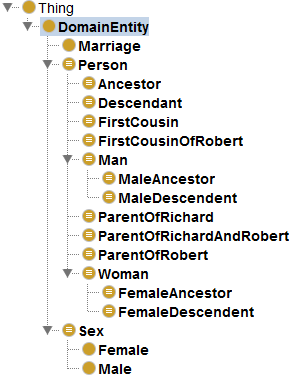
\includegraphics[width=\figwidth]{figures/class_hierarchy}\caption{A picture of the \fhkb %class hierarchy}\label{fig:tbox}
%\end{center}
%\end{figure}

\begin{figure}
\begin{center}
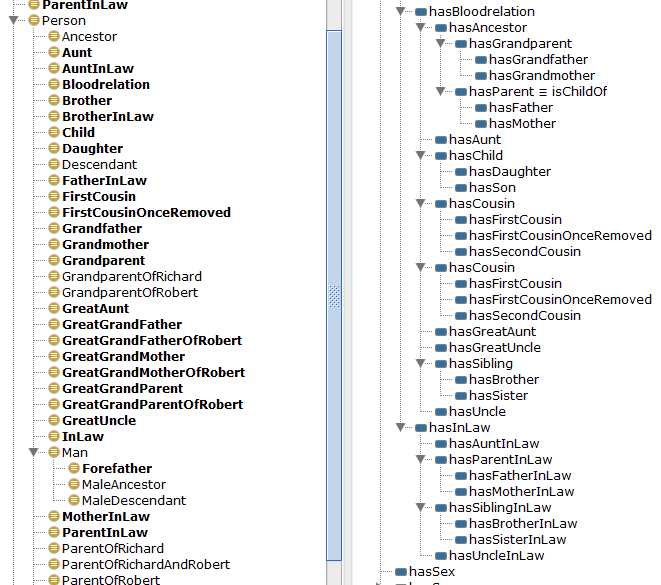
\includegraphics[width=\largefigwidth]{figures/class_prop_hierachy_final}\caption{A part of the class and property hierarchy of the final \fhkb.}\label{fig:class_and_prop_hierachy}
\end{center}
\end{figure}


%\begin{figure}
%\begin{center}
%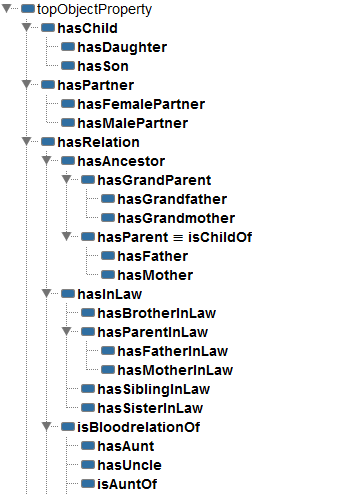
\includegraphics[width=\figwidth]{figures/new/property_hierarchy.png}\caption{A part of the final \fhkb property hierarchy.}\label{fig:proph}
%\end{center}
%\end{figure}

\section{How to use this Tutorial}

Here are some tips on using this manual to the best advantage:

\begin{itemize}
\item Start at the beginning and work towards the end.
\item You can just read  the tutorial, but building the \fhkb will help you learn much more and much more easily
\item Use the reasoner in each task; a lot of the \fhkb tutorial is about using the reasoner and not doing so will detract from the learning outcomes.
\end{itemize}


\section{\fhkb Resources}

The following resources are available at \fhkbhome :
\begin{itemize}
\item A full version of the \stevens \fhkb.
\item Some links to papers about the \fhkb.
\item Some slides about the \fhkb tutorial.
\item A set of OWL resources for each stage of the \fhkb.
\item Some blogs about the \fhkb are at \url{http://robertdavidstevens.wordpress.com}.
\end{itemize}


\section{Conventions used in this Tutorial}

\begin{itemize}
\item All OWL is written in Manchester Syntax.
\item When we use \fhkb entities within text, we use a \con{sans serif typeface}.
\item We use CamelCase for classes and property names.
\item Class names start with upper case.
\item Individual names start with a lower case letter and internal underscores to break words.
\item Property names usually start with `is' or `has' and are CamelCase with a lower case initial letter.
\item Many classes and individuals in the \fhkb have annotation properties, usually human readable labels. They show up in some of the examples in Manchester syntax, but are not made explicit as part of the tasks in this tutorial.
\item Every object property is necessarily a sub-property of topObjectProperty. It does not have to be asserted as such. Nevertheless, there might be situations where this relationship is made explicit in this tutorial for illustrative reasons.
\item The individuals we are dealing with represent distinct persons. Throughout the tutorial, once the respective axiom is introduced (chapter \ref{sec:countchildren}), the reader should make sure that all his or her individuals are always made distinct, especially when he or she adds a new one.
\item At the end of each chapter, we note the Description Logic Language (expressivity) needed to represent the ontology and the reasoning times for a number of state of the art reasoning systems. This should get the reader a sense how difficult the \fhkb becomes for reasoners to deal with over time.
\item When there is some scary OWL or the reasoner may find the \fhkb hard work, you will see a `here be dragons' image\herebedragons.\footnote{The image comes from \url{http://ancienthomeofdragon.homestead.com/} May 2012.}
\end{itemize}